\section{Experimental results}
\label{sec:experiments}

In this section, we first benchmark our continuous occlusion model for point-to-object association against the baseline method using detection bounding boxes and state-of-the-art methods for motion segmentation. We then show how the proposed model benefits the task of 3D localization in autonomous driving. For our experiments, we use the KITTI dataset~\cite{geiger2013vision}, which consists of video sequences of road scenes under a variety of driving conditions including highways and residential areas. It also provides ground truth data for different tasks such as segmentation, detection, tracking and 3D localization.

%\paragraph{Dataset} We use KITTI dataset for our experiments.  \cite{geiger2013vision}. KITTI dataset is a labeled video sequence of road scenes under variety of driving conditions including highways and residential areas in Karlsruhe, Germany. It provides manually labelled ground truth data for localization of cars and also uses velodyne data provide metrically accurate estimates of cars location.


%%%%%%%%%%%%%%%%%%%%%%%%%%%%%%%%%%%%%%%%%%%%%%%%%%%%
\subsection{Association experiment}

We first perform the association experiment that compares the accuracy of point-to-object association using the proposed model against those of the detection bounding box baseline method (BBox) and state-of-the-art motion segmentation methods, namely robust algebraic segmentation with hybrid perspective constraints (RAS)~\cite{Rao_etal_2010} and spectral clustering with point track spatial affinity (BM)~\cite{Brox_Malik_2010}.

%To verify the correctness of our association probability $\assocP$ we perform association error experiment that compare the accuracy of point track association with TPs with that of bounding box baseline method.


\subsubsection{Association results}

For each sequence of the KITTI dataset, the methods of \cite{Felzenszwalb_etal_2010} and \cite{Choi_Savarese_2010} are used respectively for computing detection bounding boxes and object tracklets. We then apply \cite{Zach2007} on object tracklets to extract point tracks. From these point tracks, we create four different sets of input point tracks, namely all point tracks, occluded point tracks, dynamic point tracks and dynamic and occluded point tracks, to examine various aspects of the methods (our method focuses on occlusion scenes while RAS and BM favour dynamic scenes). In addition to point tracks, the parameters of all TPs estimated by the method~\cite{Song_Chandraker_2014} are provided to our method (for computing association probability) and the baseline method (for depth ordering).

Figure~\ref{fig:assoc-occ-results} shows the association errors --- the percentages of point tracks incorrectly assigned to objects --- of all methods on four sets of input point tracks for each sequence of the KITTI dataset, while the mean results over all sequences are presented in Table~\ref{tab:meanAssoc}. From Figure~\ref{fig:assoc-occ-results}, our method is usually the most accurate among all methods, leading to the best mean errors on all sets of input point tracks in Table~\ref{tab:meanAssoc}, which is followed by the bounding box baseline method. This clearly shows the advantage of our continuous occlusion model over the simple baseline method for resolving occlusions. RAS and BM often have the highest errors in Figure~\ref{fig:assoc-occ-results}, and hence the highest mean errors on all sets of input point tracks in Table~\ref{tab:meanAssoc}. 

More importantly, both RAS and BM rely on motions of objects for clustering point tracks, therefore they cannot work well with static point tracks (e.g., point tracks belong to parked cars). This fact can be observed in Table~\ref{tab:meanAssoc}, where there are large differences in the mean errors of both methods on data containing static point tracks (i.e., rows 2 and 4) and data consisting of dynamic point tracks only (i.e., rows 1 and 3). In contrast, our method and the baseline method are relatively independent of object motions, resulting in smaller performance gaps.

\begin{figure*}
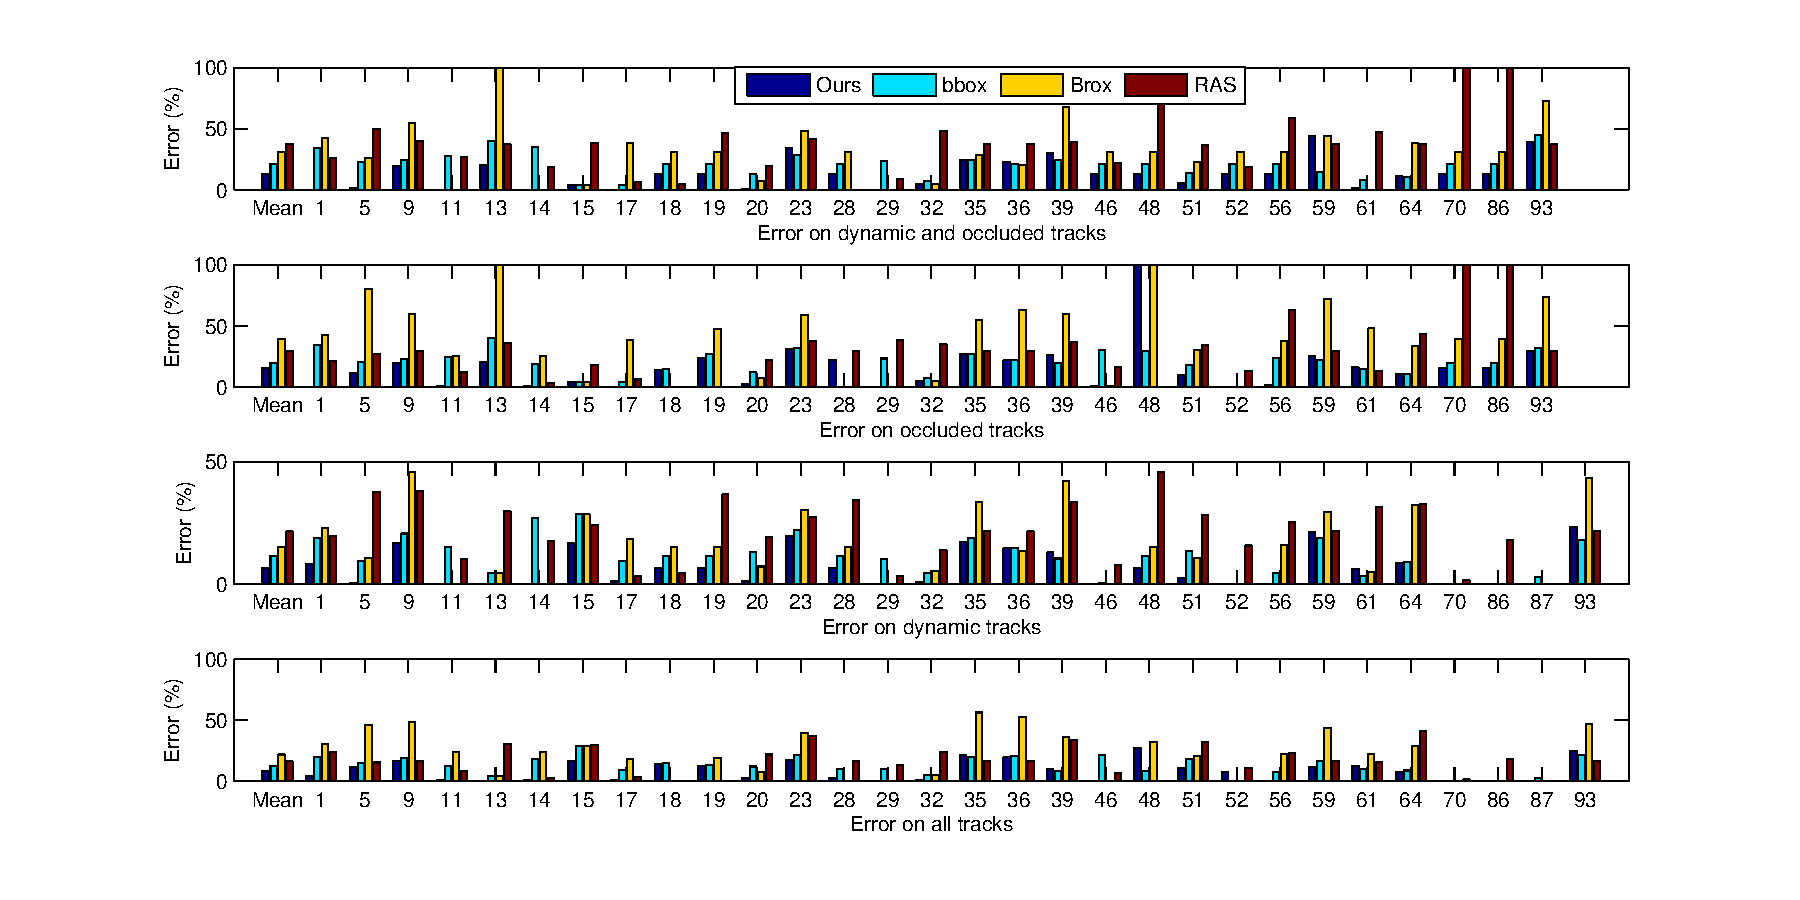
\includegraphics[trim=1.0in 0.4in 1.0in 0.2in, clip, width=\textwidth]{results/plotErrorBarEvalAssocCoeffAllSequence.pdf}
  \caption{Association errors on different sets of input point tracks. Numbers on y-axis represent data sequence numbers in KITTI dataset. Errors are in terms of average fractions of foreground points incorrectly associated to objects per sequence.}
\label{fig:assoc-occ-results}
\end{figure*}
\begin{table}
\begin{tabular}{lrrrr}
  \toprule
  & Ours & BBox & BM & RAS\\
  \midrule
  Dyn. and occ. tracks        & \textbf{13.2} & 21.3 & 30.9 & 30.1 \\
  Occluded tracks             & \textbf{15.7} & 19.8 & 39.5 & 37.8 \\
  Dynamic tracks              & \textbf{06.6} & 11.4 & 15.3 & 17.7 \\
  All tracks                  & \textbf{08.6} & 12.6 & 21.9 & 21.5 \\
  \bottomrule
\end{tabular}
\caption{Mean association errors on different sets of input point tracks over all sequences of KITTI dataset. Errors are in terms of average fractions of foreground points incorrectly associated to objects per sequence.}
\label{tab:meanAssoc}
\end{table}


\newlength{\tblimgwidth}
\setlength{\tblimgwidth}{0.40\textwidth}
\begin{table*}
  \centering
  \begin{tabular}{ccc}
    & Associations & Error in association\\
    \rotatebox{90}{\hspace{2em} BBox} & 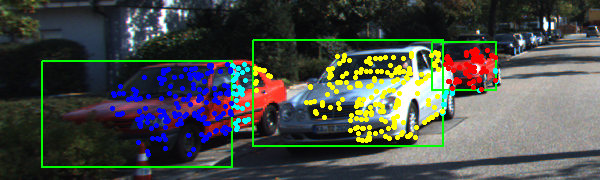
\includegraphics[width=\tblimgwidth]{results/0009_0000000060_point_assign_bbox2D_model-small.png} &%
    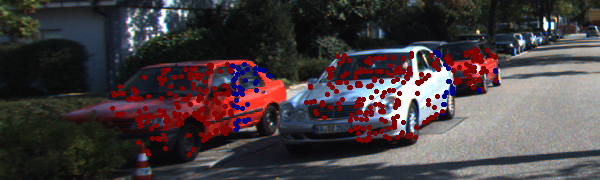
\includegraphics[width=\tblimgwidth]{results/0009_0000000060_point_assign_bbox2D_model_correct_incorrect-small.png}\\
    \rotatebox{90}{\hspace{2em} BM} & 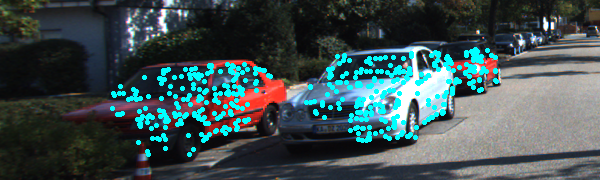
\includegraphics[width=\tblimgwidth]{results/0009_0000000060_point_assign_BroxAndMalik2010-small.png} &%
    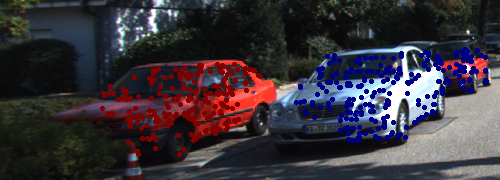
\includegraphics[width=\tblimgwidth]{results/0009_0000000060_point_assign_BroxAndMalik2010_correct_incorrect-small.png}\\
    \rotatebox{90}{\hspace{2em} RAS} & 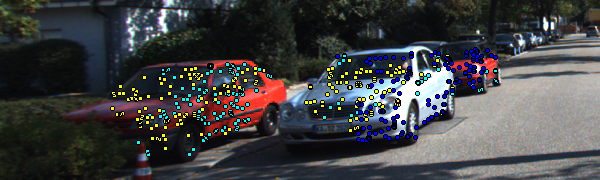
\includegraphics[width=\tblimgwidth]{results/0009_0000000060_point_assign_RAS-small.png} &%
    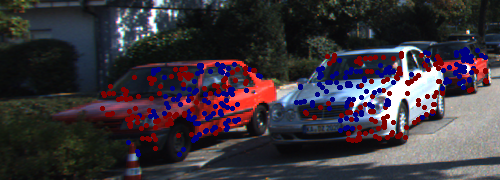
\includegraphics[width=\tblimgwidth]{results/0009_0000000060_point_assign_RAS_correct_incorrect-small.png}\\
    \rotatebox{90}{\hspace{2em} Ours} & 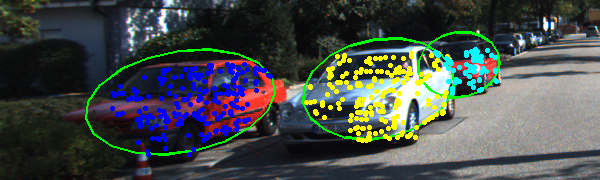
\includegraphics[width=\tblimgwidth]{results/0009_0000000060_point_assign_contPtTracks-small.png} &%
    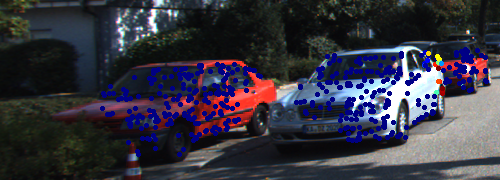
\includegraphics[width=\tblimgwidth]{results/0009_0000000060_point_assign_contPtTracks_correct_incorrect-small.png}\\
    \rotatebox{90}{\hspace{2em} BBox} & 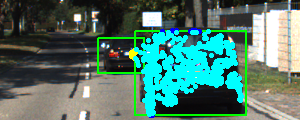
\includegraphics[width=\tblimgwidth]{results/0013_0000000060_point_assign_bbox2D_model-small.png} &%
    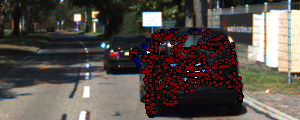
\includegraphics[width=\tblimgwidth]{results/0013_0000000060_point_assign_bbox2D_model_correct_incorrect-small.png}\\
    \rotatebox{90}{\hspace{2em} BM} & 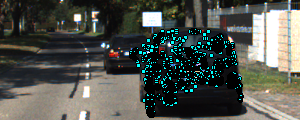
\includegraphics[width=\tblimgwidth]{results/0013_0000000060_point_assign_BroxAndMalik2010-small.png} &%
    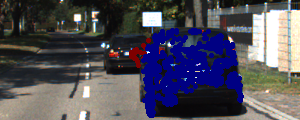
\includegraphics[width=\tblimgwidth]{results/0013_0000000060_point_assign_BroxAndMalik2010_correct_incorrect-small.png}\\
    \rotatebox{90}{\hspace{2em} RAS} & 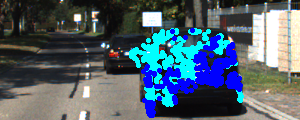
\includegraphics[width=\tblimgwidth]{results/0013_0000000060_point_assign_RAS-small.png} &%
    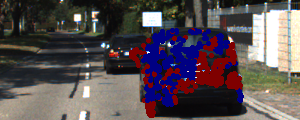
\includegraphics[width=\tblimgwidth]{results/0013_0000000060_point_assign_RAS_correct_incorrect-small.png}\\
    \rotatebox{90}{\hspace{2em} Ours} & 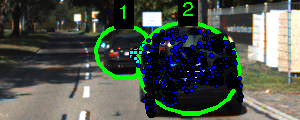
\includegraphics[width=\tblimgwidth]{results/0013_0000000060_point_assign_contPtTracks-small.png} &%
    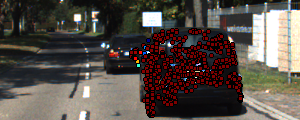
\includegraphics[width=\tblimgwidth]{results/0013_0000000060_point_assign_contPtTracks_correct_incorrect-small.png}
  \end{tabular}
  \caption{Qualitative results of the association experiment. The left column
  shows the point track assignments to appropriate objects. Each color represents
a different object to which point tracks can be associated to. Right column shows the
probabilistic error in association: low error points are in blue while high error points are in red.
Note that our method changes smoothly at the object boundaries with
intermediate probabilities, while the baseline method has merely 0-1 error.} 
\end{table*}


\begin{table}
  \centering
  \begin{tabular}{lrrr}
    \toprule
    Energy & t & yaw & dim \\
    \midrule
    initialization                                                                                  & 3.79 & \textbf{0.86} & 1.64 \\
    %$\EnergyLane+\EnergySize+\EnergyBBox+\EnergyDyn                                       $ & 3.83 & 0.90 & \textbf{1.14} \\
    %$\EnergyLane+\EnergySize+\EnergyBBoxocc+\EnergyDyn                                    $ & 3.83 & 0.90 & 1.14 \\
    %$\EnergyLane+\EnergySize+\EnergyBBoxocc+\EnergyDyn+\EnergyCol                         $ & 3.92 & 0.91 & 1.15 \\
    %$\EnergyLane+\EnergyContpttracks+\EnergySize+\EnergyBBoxocc+\EnergyDyn             $ & 3.81 & 0.92 & 1.59 \\
    % \EnergyBBox+\EnergyDyn+\EnergyCol $
    $\EnergyTrackNoOcc+\EnergyCol + \EnergyLane + \dots$  & 3.80 & 0.91 & 1.58 \\
    $\EnergyTrack+\EnergyCol + \EnergyLane + \dots$ & \textbf{3.78} & 0.91 & 1.58 \\
    \bottomrule
  \end{tabular}
  \caption{Localization experiment results with different combination of energies. We report error in three metrics translation error (t) in meters per car, yaw error (yaw) in radians per car and dimension error is again meters per car.}
  \label{tab:localizationExperiment}
\end{table}
